% 第 4 章 实鞍结开折
% 来源：docs/paper-submission/sec-general.tex（Prop. gen-scale 及改写清单）；
%       docs/paper-submission/main.tex Lemma param、Prop. saddle、Lemma res、Lemma F；
%       docs/general-statements-zh.md §1--§2.1；docs/generality-check-zh.md §1。
% 数值：figures/ch04_scales.py。

\chapter{实鞍结开折}\label{ch:unfolding}

第~\ref{ch:koenigs}、\ref{ch:fatou} 章分别处理了一个双曲不动点和一个抛物不动点。
本章把两者放进同一个单参数族：参数 $s>0$ 时有两个靠得很近的实双曲不动点，
$s=0$ 时它们合并成一个二重抛物不动点。这样的族叫做\textbf{实鞍结开折}
（real saddle-node unfolding）。从第~\ref{ch:transition} 章到第~\ref{ch:variation} 章，
全部结果都在本章的假设 (H1)--(H5) 下陈述和证明。

本章只做准备工作，不涉及分数次迭代本身。我们要回答三个定量问题：
两个乘子离 $1$ 有多远；两个 Koenigs 坐标的虚周期之差趋于什么；
用什么函数作为``两个不动点同时存在时''的近似 Abel 坐标。答案分别是
\cref{prop:scales}、\cref{lem:residues} 和模型时间 $\Psi_s$。
它们都只依赖于芽的两个系数 $a_2$、$\rho$ 和开折的一个系数 $\gamma$。

\begin{goals}
\item 实鞍结开折的定义 (H1)--(H5)，四个例子，以及 Glutsyuk 方向与 Lavaurs 方向的区别。
\item Weierstrass 预备定理把 $f_s(u)-u$ 写成二次多项式乘以无零点的因子；判别式 $D(s)=4\gamma s/a_2+O(s^2)$。
\item 尺度：$|\log\lambda_1|$、$\log\lambda_2\approx2\sqrt{a_2\gamma s}$，强迫尺度
  $\Lam=\exp\bigl(-2\pi^2/\sqrt{a_2\gamma s}\,(1+o(1))\bigr)$，内蕴参数 $p=4a_2\gamma s+O(s^2)$ 关于 $s$ 全纯。
\item 留数 $A_j=1/\log\lambda_j$ 满足 $A_1+A_2=\rho+O(s)$（它是 $s$ 的全纯函数）、$A_1(u_1-u_2)=1/a_2+O(\sqrt s)$；
  模型时间 $A_1\log(u-u_1)+A_2\log(u-u_2)$ 的一步误差是 $O(|u-u_1||u-u_2|)$，且关于 $s$ 一致。
\item tetration 的具体常数：$C_\eta=4\pi^2/\sqrt{2\ee^{1-1/\ee}}=20.3508\ldots$，以及一张数值表。
\end{goals}

% ======================================================================
\section{定义与例子}\label{ch4:sec:def}

\subsection{假设}

设 $f_s(w)$ 是一个依赖于实参数 $s$ 的映射族。我们总在一个点 $(s,w)=(0,w^*)$ 附近工作，
并取以 $w^*$ 为中心的\textbf{仿射坐标} $u$：
\begin{equation}\label{ch4:eq:affine}
 w=w^*+c\,u,\qquad c>0 .
\end{equation}
一般情形取 $c=1$；tetration 取 $c=\ee$（\cref{ch4:exa:tetration}）。在 $u$ 坐标下把 $f_s$ 写成
\[
 f_s(u):=\frac{f_s(w^*+cu)-w^*}{c}
\]
（同一个字母，按自变量的名字区分坐标）。$s=0$ 时的芽记作
\[
 g(u)=f_0(u)=u+a_2u^2+a_3u^3+\cdots .
\]

\begin{definition}[实鞍结开折]\label{def:unfolding}
称 $(f_s)_s$ 连同一个\textbf{基点}（base point）$w_0\in\R$ 为一个\textbf{实鞍结开折}
（real saddle-node unfolding），如果下列条件成立。
\begin{enumerate}[label=\textup{(H\arabic*)},leftmargin=3.2em]
\item \emph{正则性与实性.} 存在 $s_0>0$，使 $f_s(w)$ 在 $\{|s|<s_0\}\times\C$ 上对 $(s,w)$ 联合全纯，
  对每个 $s$ 是 $w$ 的整函数，并且 $s,w$ 都为实数时 $f_s(w)$ 为实数。
\item \emph{鞍结.} $f_0(w^*)=w^*$，$f_0'(w^*)=1$，且 $f_0''(w^*)>0$。在 $u$ 坐标下这就是
  \[
   a_2:=\tfrac12g''(0)=\tfrac c2f_0''(w^*)>0 .
  \]
\item \emph{横截性.} 在 $u$ 坐标下
  \begin{equation}\label{ch4:eq:direction}
   f_s=g-sX+O(s^2),\qquad X:=-\partial_sf_s\big|_{s=0},
  \end{equation}
  其中 $O(s^2)$ 在 $u$ 的一个固定圆盘上一致。函数 $X$ 叫做开折的\textbf{方向}（direction），
  数
  \[
   \gamma:=X(0)>0
  \]
  叫做\textbf{横截性常数}。
\item \emph{基点.} $w_0<w^*$，并且 $f_0$ 在 $[w_0,w^*]$ 上递增，在 $[w_0,w^*)$ 上满足 $f_0(w)>w$。
  记 $\ustar:=(w_0-w^*)/c<0$ 为基点的 $u$ 坐标。
\item \emph{非退化的 horn 映射.} $B_1\ne0$，其中 $B_n$ 是芽 $g$ 的逆上 horn 映射的 Fourier 系数
  （\cref{def:horn}）。涉及第 $n$ 个系数的对数陈述还要求 $B_n\ne0$。
\end{enumerate}
芽的\textbf{迭代留数}（iterative residue）记作
\[
 \rho:=1-\frac{a_3}{a_2^2}.
\]
$a_2,a_3,X,\gamma$，以及第~\ref{ch:fatou} 章的 Fatou 坐标、$B_n$ 与基点的 Fatou 值 $a:=\Phiatt(\ustar)$，都在 $u$ 坐标中计算。
\end{definition}

\begin{remark}[仿射坐标的选择]\label{ch4:rem:affine}
把 $c$ 换成 $c'=\mu c$（$\mu>0$），即 $u=\mu u'$，芽变成 $\mu^{-1}g(\mu u')$：$a_2\mapsto\mu a_2$，$a_3\mapsto\mu^2a_3$，$X\mapsto X(\mu\,\cdot)/\mu$，
$\gamma\mapsto\gamma/\mu$。所以 $\rho$、$a_2\gamma$ 以及乘子都与 $c$ 无关。$a$ 与 $B_n$ 的辐角依赖于 $c$，
但乘积 $B_n\ee^{2\pi\ii na}$ 与 $c$ 无关；$a$ 是实数，所以 $|B_n|$ 也与 $c$ 无关（第~\ref{ch:fatou} 章关于缩放的注）。
第~\ref{ch:transition} 章以后出现的不变量 $\tau_n$、$|B_n|$、$\Rea\kappa^{(n)}_j$ 都与 $c$ 的选取无关。
\end{remark}

\begin{remark}[符号约定]\label{ch4:rem:signs}
(H2) 中的 $a_2>0$ 与 (H3) 中的 $\gamma>0$ 都只是约定。若 $a_2<0$，用 $w\mapsto 2w^*-w$ 共轭；
若 $\gamma<0$，把 $s$ 换成 $-s$。两者都不改变问题。约定 $a_2>0$ 使吸引花瓣在 $u<0$ 一侧
（第~\ref{ch:fatou} 章），约定 $\gamma>0$ 使 $s>0$ 一侧有两个实不动点（\cref{ch4:lem:real-dynamics}）。
\end{remark}

\begin{remark}[各条假设的作用]\label{ch4:rem:roles}
\begin{enumerate}
\item (H1) 中的``整函数''只用来保证排斥不动点处的正则解 $S$ 是整函数（第~\ref{ch:transition} 章）。
  其余论证都发生在 $w^*$ 的一个固定小圆盘里，联合全纯性只在这个圆盘上用到。
  特别地，本书的局部理论\emph{不需要任何全局假设}。
\item (H3) 中的符号条件是：在 $u$ 坐标下 $\partial_sf_s(0)|_{s=0}=-\gamma<0$（在 $w$ 坐标下是 $-c\gamma$）。参数增大时，鞍结点处的值往下移。
  方向 $X$ 的其余部分 $X-X(0)$ 在第~\ref{ch:variation} 章才起作用。
\item (H4) 保证基点落在吸引不动点的直接吸引域中、并且在吸引不动点的``远侧''（\cref{ch4:lem:real-dynamics}(4)）。
  第~\ref{ch:transition} 章将看到，这正是``缝口在实轴下方半个周期''的来源。
\item (H5) 只用于比值 $t_n/t_1^n$、$c_n/c_1^n$ 和对数形式的展开。汇流定理、缝合解和不变性命题都不需要它。
\end{enumerate}
\end{remark}

\subsection{例子}

\begin{example}[tetration]\label{ch4:exa:tetration}
设 $1<b<\eta:=\ee^{1/\ee}$，$E(w)=b^w$。令
\[
 s:=1-\ee\log b .
\]
$s=0$ 时 $E(w)=\eta^w$，不动点 $w^*=\ee$，$E'(\ee)=1$。为了使芽取最简单的形式，取仿射坐标 $w=\ee(1+u)$，即 $c=\ee$。则
\[
 f_s(u)=\frac{E(\ee+\ee u)-\ee}{\ee}=\ee^{-s+(1-s)u}-1,\qquad g(u)=\ee^u-1=u+\tfrac12u^2+\tfrac16u^3+\cdots .
\]
所以 $a_2=\tfrac12$，$a_3=\tfrac16$，$\rho=1-\tfrac{1/6}{1/4}=\tfrac13$。方向是
$X(u)=-\partial_sf_s|_{s=0}=(1+u)\ee^u$，$\gamma=1$。tetration 的归一化 $F(0)=1$ 对应基点
$w_0=1$，即 $\ustar=1/\ee-1$，$a=\Phiatt(1/\ee-1)=3.0292972144180\ldots$（\cite{KneserPaper}，有区间证书）。
(H4) 成立，因为 $\eta^w$ 递增且 $w<\ee$ 时 $\eta^w>w$。
(H5) 是 \cref{prop:B1-nonzero}。$s>0$ 对应 $b<\eta$，$s<0$ 对应 $b>\eta$。
\end{example}

以后说 tetration 时，总是指 \cref{ch4:exa:tetration} 的 $u$ 坐标 $w=\ee(1+u)$。
若改用 $c=1$（$u=w-\ee$），则 $a_2=\frac1{2\ee}$、$\gamma=\ee$，$a$ 与 $B_n$ 都变，但 $B_n\ee^{2\pi\ii na}$ 不变（\cref{ch4:rem:affine}）。

\begin{example}[另外三个族]\label{ch4:exa:families}
下列三个族取自 \cite{KneserPaper} 的一般化检验（\texttt{docs/generality-check-zh.md} §1）。
\begin{enumerate}
\item \emph{二次族} $w^2+c$，$c\uparrow\frac14$。$w^*=\frac12$，$s=\frac14-c$，
  $f_s(u)=u+u^2-s$，所以 $g(u)=u+u^2$，$a_2=1$，$a_3=0$，$\rho=1$，$X\equiv1$，$\gamma=1$。
  不动点 $u_{1,2}=\mp\sqrt s$，乘子 $1\mp2\sqrt s$。基点可取 $w_0=0.2$；
  $w_0=0$（临界点）也满足 (H4)：$f_0'(w)=2w$ 只在端点 $w=0$ 处为零，$f_0$ 在 $[0,\frac12]$ 上仍严格递增。
\item \emph{正弦族} $v-\sin v+c$，$c\uparrow1$。$v^*=\pi/2$，$s=1-c$，
  $f_s(u)=u+1-\cos u-s$，$g(u)=u+\frac{u^2}2-\frac{u^4}{24}+\cdots$，所以 $a_2=\frac12$，$a_3=0$，$\rho=1$，
  $X\equiv1$，$\gamma=1$。不动点 $\arcsin c$ 与 $\pi-\arcsin c$，乘子 $1\mp\sqrt{1-c^2}$。基点取 $v_0=0.8$。
\item \emph{退化留数族} $w+(w^2-c)\ee^w$，$c\downarrow0$。$w^*=0$，$s=c$，
  $f_s(u)=u+(u^2-s)\ee^u$，$g(u)=u+u^2\ee^u$，所以 $a_2=a_3=1$，$\rho=0$，$X=\ee^u$，$\gamma=1$。
  不动点 $\mp\sqrt s$，乘子 $1-2\sqrt s\,\ee^{-\sqrt s}$ 与 $1+2\sqrt s\,\ee^{\sqrt s}$。基点取 $w_0=-0.8$。
\end{enumerate}
前两族的乘子满足 $\lambda_1+\lambda_2=2$；第三族没有这个对称性。$\rho=0$ 的芽的形式 Abel 函数没有对数项。
\end{example}

\Cref{ch4:tab:families} 汇总这些数据。最后一列是逆 horn 映射的第一个系数的模，来自
\cite[注~9.14]{KneserPaper}（数值，60 位运算）；第一行另有区间证书（\cref{ch:numerics}）。

\begin{table}[htbp]
\centering
\caption{四个实鞍结开折。$|B_1|$ 一列为数值（\texttt{generality\_check.py}）。}
\label{ch4:tab:families}
\small
\begin{tabular}{lllllll}
\toprule
族 & $s$ & $g(u)$ & $a_2$ & $\rho$ & $X$ & $|B_1|$\\
\midrule
$b^w$（$w=\ee(1+u)$） & $1-\ee\log b$ & $\ee^u-1$ & $1/2$ & $1/3$ & $(1+u)\ee^u$ & $0.0890584364122$\\
$w^2+c$ & $\tfrac14-c$ & $u+u^2$ & $1$ & $1$ & $1$ & $0.0597942361690$\\
$v-\sin v+c$ & $1-c$ & $u+1-\cos u$ & $1/2$ & $1$ & $1$ & $0.0723786416245$\\
$w+(w^2-c)\ee^w$ & $c$ & $u+u^2\ee^u$ & $1$ & $0$ & $\ee^u$ & $2744.09379131$\\
\bottomrule
\end{tabular}
\end{table}

\begin{remark}[(H5) 在各例中的状态]\label{ch4:rem:H5}
对 tetration，(H5) 是 \cref{prop:B1-nonzero}。那里的证明只用到：$g$ 限制在直接抛物吸引域上恰有一个奇异值。
二次族的直接吸引域里只有一个临界点，同一论证适用（\cite[注~9.5]{KneserPaper}）。
正弦族的临界值 $2\pi k+1$ 都是实数，只有 $k=0$ 那一个落在直接吸引域内，但 $g$ 不是有限型的，
论证能否照搬需要另外检查。对第三族，目前只有数值事实 $|B_1|\approx2744\ne0$。
所以在一般理论中，(H5) 保留为假设。
\end{remark}

\subsection{两个方向：Glutsyuk 与 Lavaurs}

一个鞍结开折在 $s=0$ 两侧的行为完全不同（\cref{ch4:lem:prep} 之后可以精确叙述）。
\begin{itemize}
\item $s>0$：两个实不动点 $u_1<u_2$，一个吸引一个排斥，乘子是 $1$ 附近的正实数。
  这是本书研究的一侧。在开折理论的文献中，沿这一侧趋于 $s=0$ 的极限称为 \textbf{Glutsyuk 方向}
  （Glutsyuk direction）：两个双曲不动点各自的线性化坐标收敛到抛物芽的两个扇形 Fatou 坐标
  \cite{Glutsyuk2001}。第~\ref{ch:confluence} 章证明的汇流定理就是这一类命题。
\item $s<0$：两个不动点是一对共轭复数，乘子 $1\pm\ii a_2\sqrt{|D(s)|}+O(s)$ 位于 $1$ 附近、
  几乎在单位圆上。实轴上的轨道从两个不动点之间的``门''穿过去。沿这一侧趋于 $s=0$ 的极限称为
  \textbf{Lavaurs 方向}，对应经典的抛物内爆（parabolic implosion）\cite{Lavaurs1989,Shishikura2000,Oudkerk1999}。
\end{itemize}
\Cref{ch4:fig:unfolding} 画出了 tetration 的 $f_s(u)-u$ 在三种 $s$ 下的图像。
对 tetration，$s<0$ 就是 $b>\eta$：Kneser 的经典构造正是在这一侧进行的。

\begin{figure}[htbp]
\centering
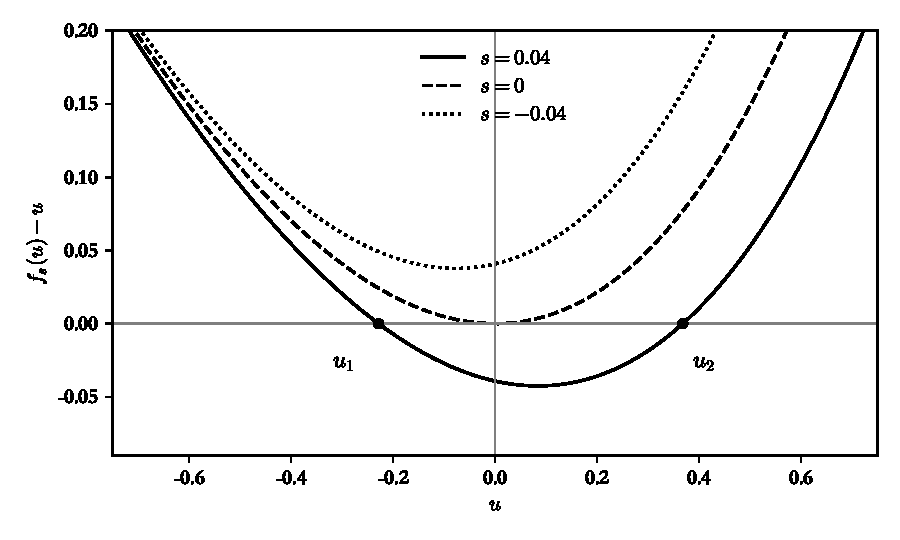
\includegraphics[width=0.7\textwidth]{figures/fig4_unfolding.pdf}
\caption{tetration 开折的 $f_s(u)-u$，$f_s(u)=\ee^{-s+(1-s)u}-1$（\texttt{figures/fig4\_unfolding.py}）。
$s=0.04$：两个实零点 $u_1=-0.2283$、$u_2=0.3683$（Glutsyuk 一侧）；$s=0$：二重零点；$s=-0.04$：没有实零点（Lavaurs 一侧）。}
\label{ch4:fig:unfolding}
\end{figure}
开折的完整解析分类（在 $0$ 的整个复邻域上）见 \cite{MRR2004,ChristopherRousseau}。
本书只在 $s>0$ 一侧工作，复参数只在第~\ref{ch:examples} 章出现。

% ======================================================================
\section{Weierstrass 预备与实动力学}\label{ch4:sec:prep}

\subsection{预备式与判别式}

记 $D_r=\{|u|<r\}$。

\begin{lemma}[预备式]\label{ch4:lem:prep}
设 (H1)--(H3) 成立。存在 $r>0$ 和 $s_1\in(0,s_0)$，使得对 $|s|<s_1$、$|u|<r$，
\begin{equation}\label{ch4:eq:prep}
 f_s(u)-u=q_s(u)\,k_s(u),\qquad q_s(u)=u^2-\beta_1(s)u+\beta_2(s),
\end{equation}
其中
\begin{enumerate}
\item $\beta_1,\beta_2$ 在 $|s|<s_1$ 上全纯，$s$ 为实数时取实值，$\beta_1(0)=\beta_2(0)=0$；
\item $k$ 在 $\{|s|<s_1\}\times\overline{D_r}$ 上联合全纯、无零点，$s,u$ 为实数时取实值，并且
  \[
   k_0(u)=a_2+a_3u+O(u^2),\qquad k_0(0)=a_2,\quad k_0'(0)=a_3 ;
  \]
\item 判别式 $D(s):=\beta_1(s)^2-4\beta_2(s)$ 满足
  \begin{equation}\label{ch4:eq:disc}
   D(s)=\frac{4\gamma}{a_2}\,s+O(s^2),\qquad \beta_2(s)=-\frac{\gamma}{a_2}s+O(s^2),\qquad \beta_1(s)=O(s).
  \end{equation}
\end{enumerate}
特别地，$f_s$ 在 $D_r$ 中恰有两个不动点（计重数），即 $q_s$ 的两个根
$u_{1,2}=\tfrac12\bigl(\beta_1\mp\sqrt{D(s)}\bigr)$，并且 $|u_j|\le C\sqrt{|s|}$。
\end{lemma}

\begin{proof}
函数 $F(s,u)=f_s(u)-u$ 在 $(0,0)$ 附近联合全纯，且 $F(0,u)=g(u)-u=u^2(a_2+a_3u+\cdots)$
在 $u=0$ 处有二阶零点。由 Weierstrass 预备定理（\cref{thm:weierstrass-prep}），
存在 $r,s_1$ 和唯一的分解 $F=q\cdot k$，其中 $q$ 是首一二次 Weierstrass 多项式，
系数在 $s=0$ 处为零，$k$ 在闭双圆盘上无零点。由唯一性，$\overline{F(\bar s,\bar u)}=F(s,u)$
推出 $q$、$k$ 都有同样的实对称性，即 (1)、(2) 中的实性。$s=0$ 时 $q_0(u)=u^2$，
所以 $k_0(u)=(g(u)-u)/u^2=a_2+a_3u+\cdots$。

在 $u=0$ 处取值：$f_s(0)=\beta_2(s)k_s(0)$。由 (H3)，$f_s(0)=g(0)-sX(0)+O(s^2)=-\gamma s+O(s^2)$；
而 $k_s(0)=a_2+O(s)$。所以 $\beta_2=-\gamma s/a_2+O(s^2)$。$\beta_1$ 全纯且 $\beta_1(0)=0$，故
$\beta_1=O(s)$，$\beta_1^2=O(s^2)$。这给出 \eqref{ch4:eq:disc}。

$k$ 无零点，所以 $D_r$ 中的不动点恰为 $q_s$ 的根。最后，$|\beta_1|\le C|s|$ 且
$|D(s)|\le C|s|$，故 $|u_j|\le C\sqrt{|s|}$（缩小 $s_1$ 使根落在 $D_{r/2}$ 内）。
\end{proof}

以后固定 \cref{ch4:lem:prep} 中的 $r$、$s_1$。由 $k$ 的连续性，可以再缩小 $r$、$s_1$，使得
\begin{equation}\label{ch4:eq:k-bounds}
 \tfrac12a_2\le|k_s(u)|\le2a_2,\qquad |k_s(u)-a_2|\le C(|s|+|u|),\qquad
 |f_s'(u)-1|\le\tfrac14
 \qquad(|s|<s_1,\ |u|<r).
\end{equation}

\subsection{$s>0$ 时的实动力学}

把 $u$ 坐标下的两个不动点换回 $w$ 坐标，记 $L=w^*+cu_1$、$L_2=w^*+cu_2$。为了记号简单，
本节的证明中取 $c=1$；一般情形只差一个正的伸缩，所有单调性与符号都不变。

\begin{lemma}[实动力学]\label{ch4:lem:real-dynamics}
设 (H1)--(H4) 成立。存在 $s_2\in(0,s_1)$，使得对每个 $s\in(0,s_2]$：
\begin{enumerate}
\item $D(s)>0$，两个不动点 $u_1<u_2$ 都是实数，$u_2-u_1=\sqrt{D(s)}$；
\item 它们的乘子
  \begin{equation}\label{ch4:eq:multipliers}
   \lambda_1=f_s'(u_1)=1-\sqrt{D}\,k_s(u_1),\qquad \lambda_2=f_s'(u_2)=1+\sqrt{D}\,k_s(u_2)
  \end{equation}
  满足 $0<\lambda_1<1<\lambda_2$；
\item $f_s$ 在实区间 $[L,L_2]$ 上严格递增，在 $(L,L_2)$ 上 $f_s(w)<w$。于是 $(L,L_2)$ 中每个点的轨道
  递减地趋于 $L$，区间 $(L,L_2)$ 落在 $L$ 的直接吸引域中；
\item $w_0<L$，$f_s$ 把 $[w_0,L)$ 映入自身，并且 $[w_0,L)$ 中每个点的轨道递增地趋于 $L$。
  特别地 $w_0$ 落在 $L$ 的直接吸引域中；
\item 设 $\sigma$ 是 $L$ 处的 Koenigs 坐标，$\sigma\circ f_s=\lambda_1\sigma$，$\sigma'(L)=1$
  （\cref{thm:koenigs}），延拓到整个吸引域上。则 $\sigma$ 在 $[w_0,L)$ 上为负，在 $(L,L_2)$ 上为正。
\end{enumerate}
\end{lemma}

\begin{proof}
(1) 由 \eqref{ch4:eq:disc}，$D(s)=\frac{4\gamma}{a_2}s(1+O(s))>0$。$\beta_j$ 实，所以两根实且相差 $\sqrt D$。

(2) 对 \eqref{ch4:eq:prep} 求导并在 $u_1$ 处取值：$f_s'(u_1)-1=q_s'(u_1)k_s(u_1)=(u_1-u_2)k_s(u_1)$；
$u_2$ 同理。由 \eqref{ch4:eq:k-bounds}，$k_s(u_j)$ 是接近 $a_2>0$ 的正实数，$\sqrt D$ 很小，
所以 $0<\lambda_1<1<\lambda_2$。

(3) 由 \eqref{ch4:eq:k-bounds}，$f_s'\ge\frac34$ 在 $D_r\cap\R$ 上成立，而 $[u_1,u_2]\subset D_r$。
在 $(u_1,u_2)$ 上 $q_s<0$、$k_s>0$，故 $f_s(u)<u$；又 $f_s(u)>f_s(u_1)=u_1$。所以
$f_s\bigl((u_1,u_2)\bigr)\subset(u_1,u_2)$，轨道单调递减、有下界 $u_1$，极限是 $[u_1,u_2)$ 中的不动点，只能是 $u_1$。
连通集 $[L,L_2)$ 落在吸引域中并含 $L$，所以落在直接吸引域中。

(4) 取 $\delta\in(0,r)$ 很小，使 $f_0(w^*-\delta)<w^*-\delta/2$（这由 $g(-\delta)=-\delta+a_2\delta^2+\cdots$ 推出）。
由 (H4)，$f_0(w)-w$ 在紧区间 $[w_0,w^*-\delta]$ 上有正的下界，$f_0$ 在其上递增，因而
$f_0([w_0,w^*-\delta])\subset(w_0,w^*-\delta/2]$。由连续性，$s$ 充分小时
$f_s(w)>w$ 在 $[w_0,w^*-\delta]$ 上成立，并且 $f_s([w_0,w^*-\delta])\subset(w_0,w^*-\delta/4)$。
再由 $|u_1|\le C\sqrt s$，$s$ 充分小时 $w^*-\delta/4<L$。另一方面，在 $[w^*-\delta,L)$ 上，
$q_s(u)>0$（$u<u_1<u_2$）、$k_s>0$，故 $f_s(w)>w$；$f_s$ 在这一段上递增，故 $f_s(w)<f_s(L)=L$。
合起来，$f_s$ 把 $[w_0,L)$ 映入 $[w_0,L)$，并且其上 $f_s(w)>w$。轨道递增有上界 $L$，极限是
$[w_0,L]$ 中的不动点；而 $[w_0,L)$ 中没有不动点，所以极限为 $L$。直接吸引域的论证同 (3)。

(5) 设 $w\in[w_0,L)$。对 $n$ 充分大，$f_s^n(w)$ 落在 $L$ 的一个小邻域里，并且 $f_s^n(w)<L$。
在这个邻域里 $\sigma$ 是实的、递增的（$\sigma'(L)=1$），$\sigma(L)=0$，所以 $\sigma(f_s^nw)<0$，
从而 $\sigma(w)=\lambda_1^{-n}\sigma(f_s^nw)<0$。对 $w\in(L,L_2)$，同样的论证给出 $\sigma(w)>0$。
\end{proof}

\begin{remark}\label{ch4:rem:far-side}
(4)、(5) 是 (H4) 的全部用处：基点在吸引不动点 $L$ 的``远离 $L_2$ 的一侧''，而线段 $(L,L_2)$
在另一侧。$\sigma$ 在两侧的符号相反，这就是第~\ref{ch:transition} 章 \cref{lem:realT} 中
$\Ima T\equiv h/2\pmod h$ 的来源。基点落在 $(L,L_2)$ 中会是什么情形，没有研究过。
\end{remark}

\subsection{反射逆}

第~\ref{ch:confluence} 章处理排斥不动点时，要把 $f_s$ 的局部逆``翻转''成一个吸引的映射。

\begin{lemma}[反射逆]\label{ch4:lem:reflected}
缩小 $r,s_1$ 后，$f_s$ 在 $D_r$ 上单叶。令
\[
 \check f_s(v):=-f_s^{-1}(-v)
\]
（$f_s^{-1}$ 取 $D_r$ 上的局部逆）。则 $\check f_s$ 对 $(s,v)$ 联合全纯，$s$、$v$ 实时取实值；
$\check f_s$ 的不动点是 $-u_2<-u_1$，前者吸引、乘子 $1/\lambda_2$，后者排斥、乘子 $1/\lambda_1$；
$s=0$ 时它的芽是
\[
 \check g(v)=v+a_2v^2+(2a_2^2-a_3)v^3+O(v^4),
\]
迭代留数为 $-\rho$。$\check f_s$ 满足 \eqref{ch4:eq:prep} 型的预备式，横截性常数仍为 $\gamma$。
\end{lemma}

\begin{proof}
由 \eqref{ch4:eq:k-bounds}，$\Rea f_s'\ge\frac34$ 在凸集 $D_r$ 上成立，故 $f_s$ 在 $D_r$ 上单叶
（Noshiro--Warschawski）；局部逆由隐函数定理对 $(s,v)$ 联合全纯。不动点和乘子直接验证。
$g^{-1}(u)=u-a_2u^2+(2a_2^2-a_3)u^3+O(u^4)$（逐阶代入 $g(g^{-1}(u))=u$），
所以 $\check g(v)=-g^{-1}(-v)=v+a_2v^2+(2a_2^2-a_3)v^3+\cdots$，迭代留数
$1-(2a_2^2-a_3)/a_2^2=-1+a_3/a_2^2=-\rho$。最后，$\check f_s(0)=-f_s^{-1}(0)$，
而 $f_s^{-1}(0)=\gamma s+O(s^2)$（由 $f_s(0)=-\gamma s+O(s^2)$ 与 $f_s'(0)=1+O(s)$），
所以 $\check f_s(0)=-\gamma s+O(s^2)$，横截性常数仍为 $\gamma$。
\end{proof}

% ======================================================================
\section{乘子与尺度}\label{ch4:sec:scales}

以下总设 $s\in(0,s_2]$，并沿用 \cref{ch4:lem:real-dynamics} 的记号。
回忆第~\ref{ch:koenigs} 章：吸引正则解 $R$ 的虚周期是 $h=2\pi/|\log\lambda_1|$，
排斥正则解 $S$ 的虚周期是 $h_2=2\pi/\log\lambda_2$。定义
\begin{equation}\label{ch4:eq:Lam-p}
 \Lam:=\exp\Bigl(\frac{4\pi^2}{\log\lambda_1}\Bigr)=\ee^{-2\pi h},\qquad
 p:=-\log\lambda_1\cdot\log\lambda_2 .
\end{equation}
$\Lam$ 叫做\textbf{强迫尺度}（forcing scale），$p$ 叫做\textbf{内蕴参数}（intrinsic parameter）。
$p$ 只依赖于两个乘子，因而在共轭和重新参数化下不变；这是用 $p$ 而不用 $s$ 作展开变量的原因
（第~\ref{ch:first-order} 章）。

为了证明 $p$ 关于 $s$ 全纯，需要一个关于对称函数的简单引理。

\begin{lemma}[根的幂和]\label{ch4:lem:power-sums}
设 $\phi(s,u)$ 在 $\{|s|<s_1\}\times\overline{D_r}$ 上联合全纯。则
\[
 \Sigma_\phi(s):=\phi(s,u_1(s))+\phi(s,u_2(s))
\]
在 $|s|<s_1$ 上全纯（$u_{1,2}(s)$ 是 $q_s$ 的两根，$s$ 为复数时也如此定义，重根计两次）。
\end{lemma}

\begin{proof}
两根都在 $D_{r/2}$ 内。由辐角原理，
\[
 \Sigma_\phi(s)=\frac1{2\pi\ii}\oint_{|u|=r}\phi(s,u)\,\frac{q_s'(u)}{q_s(u)}\,\dd u ,
\]
被积函数对 $s$ 全纯、对 $(s,u)$ 连续，且 $|u|=r$ 上 $q_s$ 无零点，所以积分对 $s$ 全纯。
\end{proof}

\begin{proposition}[尺度]\label{prop:scales}
设 (H1)--(H4) 成立。当 $s\to0^+$ 时：
\begin{enumerate}
\item 乘子满足 $\lambda_{1,2}=1\mp a_2\sqrt{D(s)}+O(s)$，并且
  \[
   |\log\lambda_1|,\ \log\lambda_2\;=\;2\sqrt{a_2\gamma s}\,\bigl(1+O(\sqrt s)\bigr);
  \]
\item 强迫尺度满足
  \[
   \Lam=\exp\Bigl(-\frac{2\pi^2}{\sqrt{a_2\gamma s}}\bigl(1+o(1)\bigr)\Bigr),
  \]
  其中 $o(1)$ 实际上是 $O(\sqrt s)$；
\item $p$ 延拓为 $|s|<s_1$ 上的全纯函数，$s$ 实时取实值，并且
  \[
   p=4a_2\gamma\,s+O(s^2);
  \]
  由于 $p'(0)=4a_2\gamma\ne0$，在 $0$ 附近 $s$ 也是 $p$ 的全纯函数，$s=p/(4a_2\gamma)+O(p^2)$；
\item $h_2-h\to2\pi\rho$。更精确地，$h_2-h=2\pi(A_1+A_2)=2\pi\rho+O(s)$，其中 $A_j=1/\log\lambda_j$。
\end{enumerate}
\end{proposition}

\begin{proof}
(1) 由 \eqref{ch4:eq:multipliers} 与 \eqref{ch4:eq:k-bounds}，$k_s(u_j)=a_2+O(|s|+|u_j|)=a_2+O(\sqrt s)$，
故 $\lambda_{1,2}=1\mp\sqrt D\,(a_2+O(\sqrt s))=1\mp a_2\sqrt D+O(s)$（$\sqrt D=O(\sqrt s)$）。
由 \eqref{ch4:eq:disc}，$\sqrt{D}=2\sqrt{\gamma s/a_2}\,(1+O(s))$，于是
$a_2\sqrt D=2\sqrt{a_2\gamma s}\,(1+O(s))$。最后 $\log(1+x)=x(1+O(x))$ 给出
$|\log\lambda_1|=a_2\sqrt D\,(1+O(\sqrt s))=2\sqrt{a_2\gamma s}\,(1+O(\sqrt s))$；$\log\lambda_2$ 同理。

(2) 由 (1)，$\log\lambda_1=-2\sqrt{a_2\gamma s}\,(1+O(\sqrt s))$，所以
\[
 \frac{4\pi^2}{\log\lambda_1}=-\frac{4\pi^2}{2\sqrt{a_2\gamma s}}\bigl(1+O(\sqrt s)\bigr)
 =-\frac{2\pi^2}{\sqrt{a_2\gamma s}}\bigl(1+O(\sqrt s)\bigr).
\]

(3) 由 \eqref{ch4:eq:k-bounds}，$|f_s'(u)-1|\le\frac14$，所以 $\ell_s(u):=\Log f_s'(u)$
（主值对数）在 $\{|s|<s_1\}\times\overline{D_r}$ 上联合全纯。对 $s\in(0,s_2]$，$\lambda_j>0$ 接近 $1$，
所以 $\log\lambda_j=\ell_s(u_j)$。于是
\[
 p=-\ell_s(u_1)\ell_s(u_2)=\tfrac12\Bigl(\Sigma_{\ell^2}(s)-\Sigma_\ell(s)^2\Bigr),
\]
其中 $\Sigma_\ell=\ell_s(u_1)+\ell_s(u_2)$，$\Sigma_{\ell^2}=\ell_s(u_1)^2+\ell_s(u_2)^2$。
由 \cref{ch4:lem:power-sums}，右边在 $|s|<s_1$ 上全纯；我们用它定义 $p$ 在整个圆盘上的延拓。
$\ell$ 的实性给出 $p$ 的实性。$s=0$ 时 $u_1=u_2=0$，$\ell_0(0)=\Log1=0$，所以 $p(0)=0$。
由 (1)，$s\to0^+$ 时 $p(s)/s=4a_2\gamma\,(1+O(\sqrt s))\to4a_2\gamma$，所以 $p'(0)=4a_2\gamma$，
而全纯性给出 $p=p'(0)s+O(s^2)$。$s$ 关于 $p$ 的全纯性是反函数定理。

(4) $h_2-h=2\pi/\log\lambda_2-2\pi/|\log\lambda_1|=2\pi(A_2+A_1)$，因为 $A_1=1/\log\lambda_1=-1/|\log\lambda_1|$。
极限 $A_1+A_2\to\rho$ 及其速率是下一节的 \cref{lem:residues}，它的证明不用 (4)。
\end{proof}

\begin{remark}\label{ch4:rem:scales}
\begin{enumerate}
\item (1) 说明两个乘子以 $\sqrt s$ 的速率离开 $1$，而且一阶上对称：$|\log\lambda_1|$ 与 $\log\lambda_2$
  只在 $O(s)$ 处不同。这一不对称性的主项由 \cref{lem:residues} 精确给出：
  $\frac1{\log\lambda_2}-\frac1{|\log\lambda_1|}=A_1+A_2\to\rho$。
\item (2) 中的 $\Lam$ 比 $s$ 的任何幂都小得多。第~\ref{ch:transition} 章将看到，
  转移映射的第 $n$ 个系数是 $\Lam^{n/2}$ 量级，分离系数 $c_n$ 是 $\Lam^n$ 量级。
\item 由 (3)，$s<0$ 时 $p$ 也有定义。那时两个乘子共轭，$\ell_s(u_2)=\overline{\ell_s(u_1)}$，
  $p=-|\ell_s(u_1)|^2<0$，与 $p\approx4a_2\gamma s$ 一致。
\end{enumerate}
\end{remark}

% ======================================================================
\section{留数与模型时间}\label{ch4:sec:residues}

\subsection{留数}

\begin{lemma}[留数]\label{lem:residues}
设 (H1)--(H4) 成立，$A_j:=1/\log\lambda_j$（于是 $A_1<0<A_2$）。当 $s\to0^+$ 时
\[
 A_1+A_2=\rho+O(s),\qquad A_1(u_1-u_2)=\frac1{a_2}+O(\sqrt s).
\]
更强地，$A_1+A_2$ 延拓为 $|s|<s_1$ 上的全纯函数 $\nu(s)$，$\nu(0)=\rho$。
因此 $A_1u_1+A_2u_2\to1/a_2$，$A_ju_j^2\to0$（$j=1,2$）。
\end{lemma}

\begin{proof}
记 $d=u_1-u_2=-\sqrt{D}$，$k_j=k_s(u_j)$。由 \eqref{ch4:eq:multipliers}，
$\lambda_1=1+dk_1$，$\lambda_2=1-dk_2$。对小的 $x$ 有
\[
 \frac1{\log(1+x)}=\frac1x+\frac12+O(x).
\]
所以
\[
 A_1=\frac1{dk_1}+\frac12+O(d),\qquad A_2=-\frac1{dk_2}+\frac12+O(d),
\]
\[
 A_1+A_2=\frac{k_2-k_1}{d\,k_1k_2}+1+O(d).
\]
由于 $k$ 关于 $(s,u)$ 联合全纯，
\[
 k_2-k_1=k_s(u_2)-k_s(u_1)=(u_2-u_1)\int_0^1\partial_uk_s\bigl(u_1+t(u_2-u_1)\bigr)\dd t
 =-d\,\bigl(a_3+O(\sqrt s)\bigr),
\]
这里用了 $\partial_uk_s(u)=k_0'(0)+O(|s|+|u|)=a_3+O(\sqrt s)$（$|u|\le C\sqrt s$）。又 $k_1k_2=a_2^2+O(\sqrt s)$。故
\[
 A_1+A_2=1-\frac{a_3}{a_2^2}+O(\sqrt s)=\rho+O(\sqrt s).
\]
其次 $A_1d=1/k_1+d/2+O(d^2)=1/a_2+O(\sqrt s)$。最后
$A_1u_1+A_2u_2=A_1(u_1-u_2)+(A_1+A_2)u_2\to1/a_2$，而 $|A_j|\le C/\sqrt s$、$u_j^2=O(s)$ 给出 $A_ju_j^2=O(\sqrt s)$。

\emph{全纯性与速率 $O(s)$.} 沿用 \cref{prop:scales}(3) 的证明中的记号 $\ell_s=\Log f_s'$、$\Sigma_\ell$。
对 $s\in(0,s_2]$，$\log\lambda_j=\ell_s(u_j)$，所以
\[
 A_1+A_2=\frac{\ell_s(u_1)+\ell_s(u_2)}{\ell_s(u_1)\ell_s(u_2)}=-\frac{\Sigma_\ell(s)}{p(s)} .
\]
$\Sigma_\ell$ 在 $|s|<s_1$ 上全纯（\cref{ch4:lem:power-sums}）且 $\Sigma_\ell(0)=2\ell_0(0)=0$；$p$ 全纯，$p(0)=0$，$p'(0)=4a_2\gamma\ne0$。
所以商在 $s=0$ 处的奇点可去（必要时缩小 $s_1$，使 $p$ 在 $0<|s|<s_1$ 上无零点），给出全纯函数 $\nu(s)$。
由上面的极限，$\nu(0)=\rho$，于是 $A_1+A_2=\rho+O(s)$。
\end{proof}

\begin{remark}\label{ch4:rem:residue-rates}
两个速率确实不同。$A_1+A_2$ 在交换两个不动点下对称，因而是 $s$ 的全纯函数，没有 $\sqrt s$ 项；
$A_1(u_1-u_2)$ 不对称，它的展开 $\frac1{k_1}+\frac d2+\cdots$ 中的 $\frac d2=-\frac12\sqrt{D(s)}$ 是真正的 $\sqrt s$ 项。
第~\ref{ch:first-order} 章的一致模型（\cref{lem:uniform-model}）也用到 $\nu(s)$ 的全纯性。
\end{remark}

\begin{example}[二次族的精确计算]\label{ch4:exa:quad-exact}
对 $f_s(u)=u+u^2-s$，$u_{1,2}=\mp\sqrt s$，$k_s\equiv1$，$\lambda_{1,2}=1\mp2\sqrt s$。令 $x=2\sqrt s$，由
$\frac1{\log(1\pm x)}=\pm\frac1x+\frac12\mp\frac x{12}+\frac{x^2}{24}+O(x^3)$，
\begin{gather*}
 A_1+A_2=1+\frac{x^2}{12}+O(x^4)=1+\frac s3+O(s^2),\\
 A_1(u_1-u_2)=\frac{-x}{\log(1-x)}=1-\frac x2+O(x^2)=1-\sqrt s+O(s).
\end{gather*}
所以 $A_1+A_2\to\rho=1$ 的速率是 $O(s)$，而 $A_1(u_1-u_2)\to1/a_2=1$ 的速率确实是 $O(\sqrt s)$（\cref{ch4:rem:residue-rates}）。
极限一步误差（\cref{ch4:lem:one-step}(3)）是
\[
 F_0(u)=-\frac1{u+u^2}+\frac1u+\log(1+u)-1=\frac1{1+u}+\log(1+u)-1=\frac{u^2}2-\frac{2u^3}3+O(u^4).
\]
\end{example}

这样 \cref{prop:scales}(4) 也证完了：$h_2-h=2\pi(A_1+A_2)=2\pi\rho+O(s)$。
对 tetration，$h_2-h\to2\pi/3$；对二次族与正弦族，$h_2-h\to2\pi$；对第三族，$h_2-h\to0$。
\cite{KneserPaper} 在 $\lambda_1=0.97$ 处测得四族的 $h_2-h$ 分别为 $2.0942$、$6.2837$、$6.2837$、$-0.0004$
（数值，\texttt{docs/general-statements-zh.md} §2.1）。

\begin{remark}[为什么留数之和是 $\rho$]\label{ch4:rem:why-rho}
考虑亚纯 $1$-形式 $\dd u/(f_s(u)-u)$。它在 $u_j$ 处的留数是 $1/(f_s'(u_j)-1)=1/(\lambda_j-1)$。
两个留数之和等于它沿 $|u|=r$ 的积分除以 $2\pi\ii$；当 $s\to0$ 时，这个积分收敛到
\[
 \frac1{2\pi\ii}\oint_{|u|=r}\frac{\dd u}{g(u)-u}
 =\frac1{2\pi\ii}\oint_{|u|=r}\frac{\dd u}{a_2u^2\bigl(1+\frac{a_3}{a_2}u+\cdots\bigr)}
 =-\frac{a_3}{a_2^2}.
\]
另一方面 $A_j=\frac1{\log\lambda_j}=\frac1{\lambda_j-1}+\frac12+O(\lambda_j-1)$，所以
$A_1+A_2=\sum_j\frac1{\lambda_j-1}+1+O(\sqrt s)\to1-\frac{a_3}{a_2^2}=\rho$。
按 \cite{Milnor2006} 的约定，$g$ 在 $0$ 处的全纯指数是 $\iota=\frac1{2\pi\ii}\oint\frac{\dd u}{u-g(u)}=\frac{a_3}{a_2^2}$（与上面的积分差一个符号），
而二重不动点的迭代留数（résidu itératif）是 $1-\iota=\rho$；$\rho$ 的名字即来自这里。习题~\ref{ch4:ex:index} 把这个论证补完整。
\end{remark}

\subsection{模型时间}

在 $s=0$ 处，第~\ref{ch:fatou} 章用形式 Abel 函数（\cref{def:formal-abel}）的前两项
\[
 \alpha_2(u):=-\frac1{a_2u}+\rho\log(-u)
\]
作为 Fatou 坐标的近似。$s>0$ 时，下面的函数起同样的作用，并且对两个不动点同时有效。

\begin{definition}[模型时间]\label{ch4:def:model-time}
对 $s\in(0,s_2]$，令
\[
 \Psi_s(u):=A_1\log(u-u_1)+A_2\log(u-u_2),
\]
它是 $D_r\setminus\{u_1,u_2\}$ 上的多值全纯函数，各分支相差 $2\pi\ii(m_1A_1+m_2A_2)$，$m_j\in\Z$。
称 $\Psi_s$ 为\textbf{模型时间}（model time）。
\end{definition}

模型时间是一个向量场的时间函数。$\Psi_s'(u)=\frac{A_1}{u-u_1}+\frac{A_2}{u-u_2}$，所以 $\Psi_s$ 是
向量场
\[
 V_s(u)=\frac1{\Psi_s'(u)}=\frac{(u-u_1)(u-u_2)}{(A_1+A_2)u-(A_1u_2+A_2u_1)}
\]
的时间坐标。$V_s$ 在 $u_j$ 处的线性部分是 $(u-u_j)/A_j=(u-u_j)\log\lambda_j$，
所以 $V_s$ 的时间一映射在两个不动点处的乘子恰好是 $\lambda_1,\lambda_2$（习题~\ref{ch4:ex:vector-field}）。
换句话说，$\Psi_s$ 是同时线性化了两个不动点的最简单的近似 Abel 坐标。
$\Psi_s$ 本身不是 $f_s$ 的 Abel 坐标；它们的偏差就是下面的一步误差。

\begin{lemma}[模型时间的极限]\label{ch4:lem:psi-limit}
设 $U\subset\C\setminus\{0\}$ 是单连通区域，$K\subset U$ 紧，$\overline U\subset D_r$ 且 $0\notin\overline U$。
对 $u,v\in K$，沿 $U$ 中同一条道路延拓 $\Psi_s$ 和 $\alpha_2$ 的对数，则当 $s\to0^+$ 时
\begin{equation}\label{ch4:eq:psilimit}
 \Psi_s(u)-\Psi_s(v)\longrightarrow\alpha_2(u)-\alpha_2(v),
\end{equation}
在 $K\times K$ 上一致，误差 $O(\sqrt s)$。
\end{lemma}

\begin{proof}
设 $\operatorname{dist}(0,U)\ge2\delta$。$s$ 小时 $|u_j|<\delta/4$，所以 $u_1,u_2\notin U$，
并且对 $u\in U$，$\bigl|\frac{u_2-u_1}{u-u_2}\bigr|\le\frac12$。写
\[
 \Psi_s(u)=(A_1+A_2)\log(u-u_2)+A_1\Log\Bigl(1+\frac{u_2-u_1}{u-u_2}\Bigr),
\]
其中第二项用主值对数。沿 $U$ 中的道路，$\log(u-u_1)$ 的连续分支等于 $\log(u-u_2)$ 的连续分支
加上这个主值对数，所以上式对 $\Psi_s$ 的任何连续分支成立（相差一个常数）。由 \cref{lem:residues}，
\[
 A_1\Log\Bigl(1+\frac{u_2-u_1}{u-u_2}\Bigr)=\frac{A_1(u_2-u_1)}{u-u_2}+O\bigl(|A_1||u_2-u_1|^2\bigr)
 =-\frac1{a_2u}+O(\sqrt s),
\]
在 $U$ 上一致。又 $(A_1+A_2)\bigl[\log(u-u_2)-\log(v-u_2)\bigr]\to\rho\bigl[\log u-\log v\bigr]$ 一致，
误差 $O(\sqrt s)$。而沿同一道路 $\log(-u)-\log(-v)=\log u-\log v$。两项相加即得 \eqref{ch4:eq:psilimit}。
\end{proof}

\subsection{一步误差}

现在估计 $\Psi_s$ 偏离 Abel 方程的程度。

\begin{lemma}[一致的一步误差]\label{ch4:lem:one-step}
存在 $r'\in(0,r)$、$s_3\in(0,s_2]$ 和 $M>0$，使得对 $s\in(0,s_3]$：
\begin{enumerate}
\item 函数
  \begin{equation}\label{ch4:eq:F}
   F_s(u):=A_1\Log\bigl(1+(u-u_2)k_s(u)\bigr)+A_2\Log\bigl(1+(u-u_1)k_s(u)\bigr)-1
  \end{equation}
  在 $\overline{D_{r'}}$ 的一个邻域上单值全纯；对 $u\in D_{r'}\setminus\{u_1,u_2\}$，它等于 $\Psi_s(f_s(u))-\Psi_s(u)-1$，
  其中 $\Psi_s(f_s(u))$ 的分支取为 $\Psi_s(u)$ 的分支加上 $\sum_jA_j\Log\frac{f_s(u)-u_j}{u-u_j}$；
\item $F_s(u_1)=F_s(u_2)=0$，并且
  \[
   |F_s(u)|\le M\,|u-u_1|\,|u-u_2|\qquad(u\in D_{r'});
  \]
\item 当 $s\to0^+$ 时，$F_s\to F_0$ 在 $D_{r'}$ 上一致，其中
  \[
   F_0(u):=\frac{k_0(u)}{a_2\bigl(1+uk_0(u)\bigr)}+\rho\Log\bigl(1+uk_0(u)\bigr)-1
   =\alpha_2(g(u))-\alpha_2(u)-1,
  \]
  这里 $\log(-g(u))-\log(-u)$ 取为 $\Log(g(u)/u)$。并且 $|F_0(u)|\le M|u|^2$。
\end{enumerate}
\end{lemma}

\begin{proof}
取 $r'$ 使 $4a_2r'\le\frac14$。由 \eqref{ch4:eq:k-bounds}，对 $u\in D_{r'}$ 及 $s$ 小，
$|(u-u_j)k_s(u)|\le2a_2(r'+|u_j|)\le\frac14$；这对 $|u|\le r'$ 成立，所以在 $\overline{D_{r'}}$ 的一个邻域上 \eqref{ch4:eq:F} 中的主值对数有定义，$F_s$ 单值全纯。

(1) 由 \eqref{ch4:eq:prep}，
\begin{equation}\label{ch4:eq:ratios}
 \frac{f_s(u)-u_1}{u-u_1}=1+(u-u_2)k_s(u),\qquad \frac{f_s(u)-u_2}{u-u_2}=1+(u-u_1)k_s(u),
\end{equation}
（因为 $f_s(u)-u_1=(u-u_1)+(u-u_1)(u-u_2)k_s(u)$），所以 $F_s$ 正是按所述分支约定的 $\Psi_s\circ f_s-\Psi_s-1$。

(2) 在 $u=u_1$ 处，第二个对数为 $\Log1=0$，第一个为 $\Log(1+(u_1-u_2)k_s(u_1))=\log\lambda_1$，
所以 $F_s(u_1)=A_1\log\lambda_1-1=0$。同理 $F_s(u_2)=A_2\log\lambda_2-1=0$。

再证 $F_s$ 在圆周 $|u|=r'$ 上一致有界。把 $F_s$ 改写成
\begin{equation}\label{ch4:eq:F-rewrite}
 F_s=A_1\Log\frac{1+(u-u_2)k_s}{1+(u-u_1)k_s}+(A_1+A_2)\Log\bigl(1+(u-u_1)k_s\bigr)-1 .
\end{equation}
（两个自变量 $1+(u-u_j)k_s$ 都在 $\{|z-1|\le\frac14\}$ 内，辐角的绝对值小于 $\pi/2$，
所以主值对数之差等于商的主值对数。）
第一个对数的自变量是 $1+\varepsilon_s(u)$，
\[
 \varepsilon_s(u)=\frac{(u_1-u_2)k_s(u)}{1+(u-u_1)k_s(u)},\qquad |\varepsilon_s(u)|\le\tfrac43\cdot2a_2|u_1-u_2| ,
\]
所以 $|A_1\Log(1+\varepsilon_s)|\le2|A_1||\varepsilon_s|\le C|A_1(u_1-u_2)|$，由 \cref{lem:residues} 有界。
第二项中 $A_1+A_2$ 有界，对数有界。所以 $|F_s|\le M_0$ 在 $D_{r'}$ 上，$M_0$ 与 $s$ 无关。

函数 $F_s(u)/\bigl((u-u_1)(u-u_2)\bigr)$ 在 $D_{r'}$ 上全纯（$u_1\ne u_2$ 处的奇点可去）。
$s$ 小时 $|u_j|\le r'/2$，所以在 $|u|=r'$ 上 $|(u-u_1)(u-u_2)|\ge(r'/2)^2$。由最大模原理，
\[
 \Bigl|\frac{F_s(u)}{(u-u_1)(u-u_2)}\Bigr|\le\frac{4M_0}{r'^2}=:M\qquad(u\in D_{r'}).
\]

(3) 在 \eqref{ch4:eq:F-rewrite} 中，$A_1\Log(1+\varepsilon_s)=A_1\varepsilon_s+O(|A_1||\varepsilon_s|^2)$，
而 $A_1\varepsilon_s=A_1(u_1-u_2)\cdot\frac{k_s(u)}{1+(u-u_1)k_s(u)}\to\frac{k_0(u)}{a_2(1+uk_0(u))}$，
$|A_1||\varepsilon_s|^2\le C|A_1(u_1-u_2)|\cdot|u_1-u_2|=O(\sqrt s)$。第二项收敛到 $\rho\Log(1+uk_0(u))$。
这些收敛在 $D_{r'}$ 上一致（用到 $k_s\to k_0$ 一致，以及 \cref{lem:residues}）。

另一方面，$g(u)=u+u^2k_0(u)=u(1+uk_0(u))$，所以
\[
 -\frac1{a_2g(u)}+\frac1{a_2u}=\frac{g(u)-u}{a_2ug(u)}=\frac{k_0(u)}{a_2(1+uk_0(u))},\qquad
 \Log\frac{g(u)}u=\Log(1+uk_0(u)),
\]
这就是 $F_0=\alpha_2\circ g-\alpha_2-1$。界 $|F_0|\le M|u|^2$ 由 (2) 中的界取极限得到。
\end{proof}

\begin{remark}\label{ch4:rem:why-alpha2}
(3) 中 $F_0=O(u^2)$ 也可以直接验证：$F_0(0)=k_0(0)/a_2-1=0$，而
\[
 F_0'(0)=\frac{k_0'(0)-k_0(0)^2}{a_2}+\rho\,k_0(0)=\frac{a_3}{a_2}-a_2+a_2-\frac{a_3}{a_2}=0 .
\]
一次项的抵消恰好要求对数项的系数是 $\rho=1-a_3/a_2^2$。这是在 $\alpha$ 中出现 $\rho\log(-u)$ 的原因（\cref{def:formal-abel}）。
\cref{ch4:lem:one-step} 说明：$s>0$ 时，同样的抵消在两个不动点处同时发生，而且误差关于 $s$ 一致。
这是第~\ref{ch:confluence} 章汇流定理的核心估计；第~\ref{ch:first-order} 章的一致模型（\cref{lem:uniform-model}）
把 $\Psi_s$ 加上多项式修正，使误差变成 $O(|q_s|^N)$。
\end{remark}

\subsection{模型时间给出 Abel 坐标}

一步误差的用处是：把它沿轨道加起来，就把模型时间修正成真正的 Abel 坐标。对固定的 $s>0$ 这很容易，
因为轨道以几何速率趋于 $u_1$。设 $\sigma$ 是 $L$ 处的 Koenigs 坐标（\cref{ch4:lem:real-dynamics}(5)），
$R$ 是以 $w_0$ 为初值的吸引正则解（\cref{def:regular-solution}）。它的逆，即吸引 Abel 坐标，是多值函数
\begin{equation}\label{ch4:eq:Rinv}
 R^{-1}(w)=\frac{\log\bigl(\sigma(w)/\sigma(w_0)\bigr)}{\log\lambda_1},
\end{equation}
各分支相差 $\ii h\Z$（第~\ref{ch:transition} 章将正式讨论）。

\begin{lemma}[由模型时间构造吸引 Abel 坐标]\label{ch4:lem:model-abel}
固定 $s\in(0,s_3]$。设 $B\subset D_{r'}$ 是以 $u_1$ 为心的开圆盘，$u_2\notin\overline B$，且在 $B$ 上 $|f_s'|\le\theta<1$。则
\begin{enumerate}
\item $H_s:=\sum_{k\ge0}F_s\circ f_s^k$ 在 $B$ 上一致收敛到全纯函数，$H_s(u_1)=0$；
\item 记 $\mathcal A_s:=\Psi_s+H_s$，$\sigma_u(u):=\sigma(w^*+cu)$。在 $B\setminus\{u_1\}$ 的任何单连通子区域上，
  对 $\Psi_s$ 与 $\log\sigma_u$ 的任何连续分支，$\mathcal A_s-A_1\log\sigma_u$ 是常数；
\item 因此，若 $u,v\in B\setminus\{u_1\}$，则沿 $B\setminus\{u_1\}$ 中同一条道路取分支，
  \[
   R^{-1}(w^*+cu)-R^{-1}(w^*+cv)=\mathcal A_s(u)-\mathcal A_s(v)\pmod{\ii h} .
  \]
\end{enumerate}
\end{lemma}

\begin{proof}
(1) $B$ 是凸的，$|f_s'|\le\theta$，且 $f_s(u_1)=u_1$，所以 $|f_s^k(v)-u_1|\le\theta^k|v-u_1|$，$f_s^k(B)\subset B$。
由 \cref{ch4:lem:one-step}(2)，$|F_s(f_s^kv)|\le M\,\operatorname{diam}(D_{r'})\,\theta^k|v-u_1|$，级数一致收敛。$F_s(u_1)=0$ 给出 $H_s(u_1)=0$。

(2) 导数是单值的。由 $F_s=\Psi_s\circ f_s-\Psi_s-1$ 得 $F_s'=\Psi_s'(f_s)f_s'-\Psi_s'$；由 $H_s\circ f_s=H_s-F_s$ 得
$H_s'(f_s)f_s'=H_s'-F_s'$。相加：
\[
 \mathcal A_s'(f_s(u))\,f_s'(u)=\mathcal A_s'(u).
\]
同理，$\omega:=\sigma_u'/\sigma_u$ 满足 $\omega(f_s(u))f_s'(u)=\omega(u)$（对 $\sigma_u\circ f_s=\lambda_1\sigma_u$ 取对数导数）。
$f_s$ 在 $D_r$ 上单叶（\cref{ch4:lem:reflected}），所以 $\sigma_u$ 在 $B$ 中只有一个零点 $u_1$，且是单零点
（若 $\sigma_u(v)=0$，则 $f_s^n(v)$ 是 $u_1$ 附近 $\sigma_u$ 的零点，只能是 $u_1$，再由单叶性 $v=u_1$）。
于是 $\omega$ 与 $\Psi_s'=\frac{A_1}{u-u_1}+\frac{A_2}{u-u_2}$ 在 $u_1$ 处都是单极点，留数分别为 $1$ 与 $A_1$，
所以 $E:=\mathcal A_s'-A_1\omega$ 在 $B$ 上全纯，并满足 $E(f_s(u))f_s'(u)=E(u)$。迭代得
$E(u)=E(f_s^nu)\,(f_s^n)'(u)$。在比 $B$ 略小的同心闭圆盘 $\overline{B'}$ 上（它也被 $f_s$ 映入自身），$E$ 有界，而 $|(f_s^n)'|\le\theta^n\to0$，
所以 $E\equiv0$ 于 $B'$，从而于 $B$。故 $\mathcal A_s-A_1\log\sigma_u$ 的导数为零。

(3) 由 \eqref{ch4:eq:Rinv}，$R^{-1}(w^*+cu)-R^{-1}(w^*+cv)=A_1\bigl(\log\sigma_u(u)-\log\sigma_u(v)\bigr)$，
它在分支的意义下确定到 $2\pi\ii A_1\Z=\ii h\Z$。再用 (2)。
\end{proof}

基点 $\ustar$ 一般不在 $B$ 中（$B$ 很小，$\ustar$ 是固定的负数）。对吸引域中的一般点，用函数方程 $R^{-1}(f_s(w))=R^{-1}(w)+1$
把轨道推进 $B$：若 $f_s^n(u)\in B$、$f_s^{n_0}(\ustar)\in B$（都不等于 $u_1$），则
\[
 R^{-1}(w^*+cu)=\mathcal A_s\bigl(f_s^n(u)\bigr)-n-\mathcal A_s\bigl(f_s^{n_0}(\ustar)\bigr)+n_0\pmod{\ii h},
\]
这里 $f_s^n$ 是 $f_s$ 在整个 $u$ 平面上的迭代（(H1)），分支沿 (3) 中的道路取。

\begin{remark}[困难在于一致性]\label{ch4:rem:uniformity}
\cref{ch4:lem:model-abel} 中的 $\theta$ 必须小于 $1$，而 $\theta\ge\lambda_1\to1$（$s\to0$）。圆盘 $B$ 也随 $s\to0$ 缩成一点。
所以这个引理对 $s\to0$ 毫无用处：它给出的级数在 $s\to0$ 时不一致收敛。
第~\ref{ch:confluence} 章的做法是换一个区域：在 Apollonius 圆盘 $\{\Rea A_1\log\frac{u-u_1}{u-u_2}>R\}$ 上，
\cref{ch4:lem:one-step} 的二次界 $|F_s|\le M|u-u_1||u-u_2|$ 沿轨道的和关于 $s$ 一致地被 $C/R$ 控制（\cref{lem:petal}），
而当 $s\to0$ 时这些圆盘收敛到抛物花瓣 $\{\Rea(-1/(a_2u))>R\}$。那时 $\mathcal A_s$ 的极限就是 $\alpha_2+\sum_kF_0\circ g^k$，
即吸引 Fatou 坐标。这正是汇流定理的机制。
\end{remark}

% ======================================================================
\section{tetration 的具体常数}\label{ch4:sec:tetration}

\begin{lemma}[乘子参数化]\label{ch4:lem:tet-param}
设 $1<b\le\eta$。$E(w)=b^w$ 的不动点 $L$ 的乘子 $\lambda=L\log b$ 满足
$L=\ee^\lambda$ 与 $\log b=\lambda\ee^{-\lambda}$。函数 $\lambda\mapsto\lambda\ee^{-\lambda}$ 在 $(0,1)$ 上递增、
在 $(1,\infty)$ 上递减，最大值 $\ee^{-1}=\log\eta$。因此 $\lambda_1\in(0,1)$ 与 $\lambda_2\in(1,\infty)$
分别通过吸引与排斥不动点参数化 $(1,\eta)$，两支在 $b=\eta$ 处相遇，并且
\[
 s=1-\ee\log b=1-\lambda_j\ee^{1-\lambda_j}\qquad(j=1,2).
\]
\end{lemma}

\begin{proof}
$L=b^L$ 给出 $\log L=L\log b=\lambda$。其余是 $\frac{\dd}{\dd\lambda}(\lambda\ee^{-\lambda})=(1-\lambda)\ee^{-\lambda}$。
\end{proof}

记 $\lambda_1=1-\delta$。展开 $(1-\delta)\ee^\delta=1-\frac{\delta^2}2-\frac{\delta^3}3-\frac{\delta^4}8+O(\delta^5)$，得
$s=\frac{\delta^2}2+\frac{\delta^3}3+O(\delta^4)$，与 \cref{prop:scales}(1)（$a_2=\frac12$、$\gamma=1$，
$|\log\lambda_1|\approx\sqrt{2s}$）一致。由 \cref{prop:scales}(3)，$p=2s+O(s^2)$；
更精确的展开是 $p=2s+\frac{10}9s^2+\frac79s^3+O(s^4)$（习题~\ref{ch4:ex:tet-p}）。

\begin{corollary}[tetration 的强迫尺度]\label{ch4:cor:ceta}
当 $b\to\eta^-$ 时，
\[
 \Lam=\exp\Bigl(-\frac{C_\eta}{\sqrt{\eta-b}}\bigl(1+o(1)\bigr)\Bigr),\qquad
 C_\eta=\frac{4\pi^2}{\sqrt{2\ee^{1-1/\ee}}}=20.3508008134\ldots
\]
\end{corollary}

\begin{proof}
由 \cref{prop:scales}(2)，$-\log\Lam=\frac{2\pi^2}{\sqrt{s/2}}(1+o(1))=\frac{2\sqrt2\pi^2}{\sqrt s}(1+o(1))$。
又 $s=\ee(\log\eta-\log b)=\frac{\ee}{\eta}(\eta-b)\bigl(1+O(\eta-b)\bigr)$，所以
\[
 -\log\Lam=\frac{2\sqrt2\,\pi^2\sqrt{\eta/\ee}}{\sqrt{\eta-b}}\bigl(1+o(1)\bigr),\qquad
 2\sqrt2\,\pi^2\sqrt{\eta/\ee}=2\sqrt2\,\pi^2\ee^{(1/\ee-1)/2}=\frac{4\pi^2}{\sqrt{2\ee^{1-1/\ee}}} .\qedhere
\]
\end{proof}

\begin{example}[数值]\label{ch4:exa:numbers}
\Cref{ch4:tab:tet} 列出 tetration 在几个 $\lambda_1$ 处的尺度（脚本 \texttt{figures/ch04\_scales.py}，mpmath 40 位）。
可以看到：$|\log\lambda_1|/\sqrt{2s}-1$ 按 $O(\sqrt s)$ 缩小，主项是 $\frac{\sqrt2}6\sqrt s$（习题~\ref{ch4:ex:tet-p} 的方法可以算出）；$p/s\to2=4a_2\gamma$，
偏差约为 $\frac{10}9s$；$h_2-h\to2\pi/3=2.0943951\ldots$；$A_1+A_2\to\frac13$ 与 $A_1(u_1-u_2)\to2=1/a_2$
的速率不同：前者是 $O(s)$（数值上 $(A_1+A_2-\frac13)/s\approx-0.0037037$），后者是 $O(\sqrt s)$，并且在 $\lambda_1\in[0.5,0.9]$ 上还不单调（\cref{ch4:rem:residue-rates}）。最后一列是 $-\sqrt{\eta-b}\,\log\Lam$，
它以 $O(\sqrt s)$ 的速率趋于 $C_\eta=20.3508\ldots$。$\Lam$ 极小：$\lambda_1=0.9$ 时已是 $10^{-163}$ 量级。
\end{example}

\begin{table}[htbp]
\centering
\caption{tetration 的尺度（数值，\texttt{figures/ch04\_scales.py}）。$u_j=\ee^{\lambda_j-1}-1$。}
\label{ch4:tab:tet}
\small\setlength{\tabcolsep}{2.5pt}
\begin{tabular}{lllllllll}
\toprule
$\lambda_1$ & $s$ & $\lambda_2$ & $\frac{|\log\lambda_1|}{\sqrt{2s}}$ & $p/s$ & $\Lam$ & $h_2-h$ & $A_1+A_2$ & $-\sqrt{\eta-b}\log\Lam$\\
\midrule
$0.5$ & $0.175639$ & $1.756431$ & $1.169498$ & $2.22296$ & $1.8\times10^{-25}$ & $2.08984$ & $0.3326083$ & $17.1240$\\
$0.8$ & $0.0228778$ & $1.230842$ & $1.043187$ & $2.02583$ & $1.5\times10^{-77}$ & $2.09386$ & $0.3332475$ & $19.4673$\\
$0.9$ & $5.34617\times10^{-3}$ & $1.107147$ & $1.018923$ & $2.00596$ & $1.9\times10^{-163}$ & $2.09427$ & $0.3333135$ & $19.9630$\\
$0.95$ & $1.29246\times10^{-3}$ & $1.051724$ & $1.008875$ & $2.00144$ & $5.5\times10^{-335}$ & $2.09437$ & $0.3333285$ & $20.1694$\\
$0.99$ & $5.03346\times10^{-5}$ & $1.010067$ & $1.001688$ & $2.00006$ & $1.2\times10^{-1706}$ & $2.09439$ & $0.3333332$ & $20.3164$\\
$0.999$ & $5.00333\times10^{-7}$ & $1.001001$ & $1.000167$ & $2.000001$ & $2.1\times10^{-17137}$ & $2.09440$ & $0.3333333$ & $20.3474$\\
\bottomrule
\end{tabular}
\end{table}

$A_1(u_1-u_2)$ 在上表六个点处的值依次为 $2.19885$、$1.97599$、$1.97664$、$1.98576$、$1.99676$、$1.99967$。
\cite{KneserPaper} 在 $\lambda_1=0.99$ 处给出的 $A_1+A_2=0.3333331469$ 和 $A_1(u_1-u_2)=1.99676$ 与本表一致。

% ======================================================================
\notes

\textbf{来源.} 本章是 \cite{KneserPaper} 中 General real saddle-node unfoldings 一节（Setting 与 命题~9.1）
的展开，并把指数族写死的常数一律换成一般形式：论文中的 $\frac12$、$\frac13$、$-2/u$、$p'(0)=2$
分别换成 $a_2$、$\rho$、$-1/(a_2u)$、$4a_2\gamma$。\cref{prop:scales} 对应论文 引理~2.1、命题~2.2
与 命题~9.1；\cref{lem:residues} 与 \cref{ch4:lem:one-step} 对应论文 引理~4.1 与 引理~4.2
（论文中写作 $\nu=1-4k_\eta'(0)=\frac13$ 与 $A_1(u_1-u_2)\to2$）。论文的 命题~9.1 只写了 $p$ 关于 $s$ 全纯；
这里用根的幂和（\cref{ch4:lem:power-sums}）给出了一个完整的证明。论文 (H3) 中的 $\gamma=\partial_\mu f_\mu(w^*)$
与 $s=\mu_0-\mu$ 合起来就是本章的 $X(0)=-\partial_sf_s(0)=\gamma$（论文取 $c=1$；一般的 $c$ 下本章的 $\gamma$ 是论文的 $\gamma$ 除以 $c$）。
$A_1+A_2$ 的全纯性与速率 $O(s)$（\cref{lem:residues}）论文中没有单独陈述。
(H4) 的推论 \cref{ch4:lem:real-dynamics}(4)(5) 在论文中只陈述未证明，这里补全了。

\textbf{鞍结开折.} 抛物不动点的开折是一个经典题目。Lavaurs 方向的抛物内爆见 \cite{Lavaurs1989,Shishikura2000,Oudkerk1999}；
Glutsyuk 方向的汇流见 \cite{Glutsyuk2001}；对一般（复）参数的解析分类见
Marde\v{s}i\'c--Roussarie--Rousseau \cite{MRR2004} 与 Christopher--Rousseau \cite{ChristopherRousseau}，
向量场情形见 \cite{RousseauTeyssier2008}，可和性见 \cite{Ribon2010}。
这些文献中最常用的开折参数是``标准形''参数，本书则用乘子构造的 $p$。两者都关于 $s$ 全纯，
彼此差一个全纯的重新参数化；本书的结果只依赖于乘子，因此可以不经标准形直接陈述。

\textbf{模型时间.} 函数 $A_1\log(u-u_1)+A_2\log(u-u_2)$ 是向量场 $V_s$ 的时间。
用一个有两个零点的模型向量场的时间来近似开折的 Fatou 坐标，是开折分类理论中的标准做法
（参看 \cite{MRR2004}）。本书的写法让两个留数 $A_1,A_2$ 分别出现，
便于证明 \cref{ch4:lem:one-step} 中``误差在两个不动点处同时为零''。

\textbf{迭代留数.} $\rho=1-a_3/a_2^2$ 是芽在切于恒等的共轭下的形式不变量。
它在复动力系统中以 résidu itératif 之名出现（\cite{Milnor2006}；关于它在 horn 映射上的类比，见 \cite{BuffEpstein2002}）。

% ======================================================================
\exercises

\begin{exercise}\label{ch4:ex:quad}
对二次族 $w^2+c$，直接验证 \cref{ch4:exa:families} 中的数据，并证明 $p=-\log(1-2\sqrt s)\log(1+2\sqrt s)$
满足 $p=4s+\frac{20}3s^2+O(s^3)$。它关于 $s$ 全纯吗？
\end{exercise}
\begin{hint}
$-\log(1-x)\log(1+x)=x^2+\frac5{12}x^4+O(x^6)$ 是 $x$ 的偶函数。
\end{hint}

\begin{exercise}\label{ch4:ex:expq-prep}
对第三族 $w+(w^2-c)\ee^w$，写出预备式 \eqref{ch4:eq:prep} 中的 $q_s$ 与 $k_s$，验证 $D(s)=4s=4\gamma s/a_2$，
并计算 $\lambda_1,\lambda_2$ 与 $A_1+A_2$ 的前两项。说明为什么 $\lambda_1+\lambda_2\ne2$。
\end{exercise}

\begin{exercise}\label{ch4:ex:rho-invariant}
设 $\phi(u)=\mu u+du^2+O(u^3)$，$\mu>0$。证明 $\phi^{-1}\circ g\circ\phi$ 的前两个系数为
$\tilde a_2=\mu a_2$、$\tilde a_3=\mu^2a_3$（二次项系数 $d$ 不出现），从而 $\tilde\rho=\rho$。
再说明 $\gamma$ 在坐标伸缩 $u\mapsto\mu u$ 与参数伸缩 $s\mapsto\kappa s$（$\kappa>0$）下如何变化；
证明 $4a_2\gamma$ 在前者下不变，在后者下乘以 $1/\kappa$。
\end{exercise}
\begin{hint}
$4a_2\gamma=p'(0)$，而 $p$ 只依赖于乘子。
\end{hint}

\begin{exercise}\label{ch4:ex:H4}
对 \cref{ch4:exa:families} 中的三个族验证 (H4)。对第三族，证明 $f_0'(w)=1+(w^2+2w)\ee^w\ge0.53$ 在 $[-0.8,0]$ 上成立。
\end{exercise}

\begin{exercise}\label{ch4:ex:lavaurs}
设 $s<0$。证明 $f_s$ 在 $D_r$ 中的两个不动点是一对共轭复数，乘子 $\lambda,\bar\lambda$ 满足
$\lambda=1+\ii a_2\sqrt{|D(s)|}+O(s)$。对二次族，证明 $c>\frac14$ 时两个不动点都是排斥的。
\end{exercise}

\begin{exercise}\label{ch4:ex:vector-field}
验证模型时间 $\Psi_s$ 是向量场 $V_s$ 的时间坐标，并证明 $V_s$ 的时间一映射 $\exp(V_s)$ 在 $u_j$ 处的乘子等于 $\lambda_j$。
$\exp(V_s)$ 在 $u_j$ 之外还有其他不动点吗？
\end{exercise}
\begin{hint}
在 $u_j$ 附近 $V_s(u)=(u-u_j)\log\lambda_j+O((u-u_j)^2)$。
\end{hint}

\begin{exercise}\label{ch4:ex:index}
补完 \cref{ch4:rem:why-rho} 的论证：证明 $\sum_j\frac1{\lambda_j-1}=\frac1{2\pi\ii}\oint_{|u|=r'}\frac{\dd u}{f_s(u)-u}$，
令 $s\to0$，并由此给出 $A_1+A_2\to\rho$ 的另一个证明。说明右边的积分是 $s$ 的全纯函数，并由此再得到 \cref{lem:residues} 中的速率 $O(s)$。
\end{exercise}

\begin{exercise}\label{ch4:ex:tet-p}
对 tetration，令 $\lambda_1=1+x_1$、$\lambda_2=1+x_2$，它们是 $1-(1+x)\ee^{-x}=s$ 的两个根。
证明 $p=2s+\frac{10}9s^2+\frac79s^3+O(s^4)$，并用 \cref{ch4:tab:tet} 核对前两项。
\end{exercise}
\begin{hint}
令 $s=t^2$，把 $x_{1,2}$ 展成 $t$ 的幂级数（$x_2(t)=x_1(-t)$），再展开 $-\log(1+x_1)\log(1+x_2)$。
\end{hint}

\begin{exercise}\label{ch4:ex:F0}
对 $g(u)=\ee^u-1$，计算 $F_0(u)=\alpha_2(g(u))-\alpha_2(u)-1$ 的 $u^2$ 项系数。对一般芽，用 $a_2,a_3,a_4$ 表示这个系数。
\end{exercise}

\begin{exercise}\label{ch4:ex:reflected}
设 $g(u)=u+u^2$。写出 $\check g$ 的前四项，验证其迭代留数为 $-1$，并解释：为什么 $\check g$ 的吸引花瓣对应 $g$ 的排斥花瓣。
\end{exercise}

\begin{exercise}\label{ch4:ex:uniform-rate}
证明 \cref{ch4:lem:one-step}(3) 中的收敛有速率：$\sup_{D_{r'}}|F_s-F_0|=O(\sqrt s)$。
再对二次族数值计算 $\sup_{|u|=0.1}|F_s-F_0|$，观察到它实际上是 $O(s)$，尽管 $A_1(u_1-u_2)$ 含 $\sqrt s$ 项。解释原因。
\end{exercise}
\begin{hint}
第一问用 \cref{lem:residues} 与 $|u_j|\le C\sqrt s$。第二问：$F_s$ 在交换 $(u_1,A_1)\leftrightarrow(u_2,A_2)$ 下不变；
第~\ref{ch:first-order} 章 \cref{lem:uniform-model}（取 $N=1$）证明 $F_s$ 对 $s$ 全纯，所以 $F_s-F_0=O(s)$。
\end{hint}
